\normalfont\normalsize
\chapter{Hardware Platform}

This chapter presents the hardware platforms used by the solution proposed in this thesis. 

Because we wanted to create not only a way of acquiring data from WSNs in remote locations, but also a simple and low cost solution, we selected the Parrot AR.Drone 2.0 as our work horse. The drone carries the mobile gateway which communicates with the nodes of the Sparrow sensors family. The drone provides several key features required by our solution, such as an embedded Linux system, a mobile platform with the possibility of autonomous flying and sufficient flight time.

In order to keep the price low and the footprint small, the Sparrow family uses a surface mounted antenna. The antenna has a gain of -1 dBi and it is perfect for applications were size is a constraint. When size can be overlooked, the range of the device can be extended by mounting an external antenna.

The cost of our solution depends on the configuration and size of the WSN islands. As previously mentioned the drone costs 300\$, the price for one node is 35\$, and the dongle is 45\$ . A high gain replacement antenna for the Sparrow nodes can cost 8\$.

Example costs for two different types of networks:
\begin{itemize}

\item An area that needs a high density of nodes and covers a small surface does not require the nodes to have an external antenna. The system will be comprised of a drone, one dongle with an external antenna and 10 nodes. The total cost would amount to approximately 700\$.

\item  An area that needs a low density of nodes, but covers a larger surface, or are placed in high vegetation or in a high interference area will require the nodes to be equipped with an external antenna.  The system will be comprised of a drone, one dongle with an external antenna and 10 nodes, also with external antennas. The total cost would amount to approximately 800\$.

\end{itemize}

\section{The Parrot AR.Drone 2.0}

Figure~\ref{fig:drone} shows Parrot AR.Drone, a Wi-Fi radio controlled quad-copter built by the French company Parrot\cite{parrot2012drone} .
The original drone was released in 2010 and in 2012 it was replaced by version 2.0. Since the launch of the original AR.Drone, more the half a million units have been sold, making it one of the, if not, the most popular drone on the market \cite{parrotpopular}. The reason of its success is not entirely due to the relatively low price, but also because of its embedded Linux system and integrated USB port that can accommodate any device using that interface which is compatible with the Linux operating system. This makes the drone an incredibly versatile platform and can be very easily integrated with different systems. 
\begin{figure}[ht]
\begin{center}
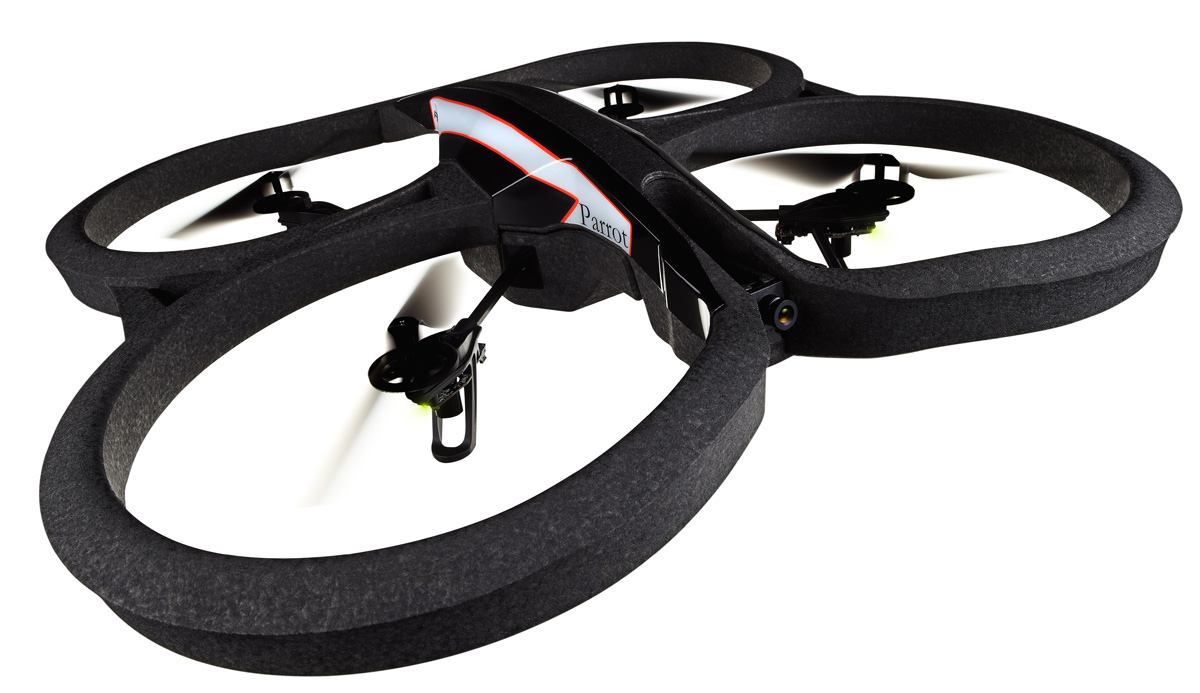
\includegraphics[width=0.9\textwidth]{img/drone.jpg}
\end{center}
\caption{\small \itshape{The Parrot AR.Drone 2.0}}
  \label{fig:drone}
\end{figure}

\footnotetext{Image taken from \cite{parrot_drone}}

Because of its popularity and versatility the Drone has a number of after-market modules that can be attached to it, such as 
the Flight Recorder GPS Module. This module has a built-in storage of 4GB for video recording purposes and a built in GPS receiver. This allows the drone to follow a predetermined path of waypoints and to return back from where it took off automatically, all within the limits of the Wi-Fi connection with the controlling device.

In order to properly accommodate the SparrowDongle, the hull had to be modified . The required external antenna of the dongle was mounted on top of the polyester cover and a small counterweight has been glued at the opposite side of the dongle. The counterweight acts as a stability ballast that keeps the drone leveled while flying and can be seen in figure~\ref{fig:counterweight}.

The Parrot AR.Drone 2.0 has the following specifications:
\begin{itemize}
\item   1GHz, 32 bit ARM Cortex A8 processor at 800MHz
\item   video DSP TMS320DMC64x
\item   Linux 2.6.32 kernel
\item   1GB DDR2 RAM at 200MHz
\item   USB 2.0 high speed for extensions
\item   Wi-Fi b,g,n
\item   3 axis gyroscope with 2000°/second precision
\item   3 axis accelerometer with $\pm$50mg precision
\item   3 axis magnetometer with $\pm$6° precision
\item   Pressure sensor with $\pm$10 Pa precision
\item   Ultrasound sensors for ground altitude measurement
\item   60 fps vertical QVGA camera for ground speed measurement
\item	30 fps 720p front mounted camera 	
\end{itemize}

\begin{figure}[ht]
\begin{center}
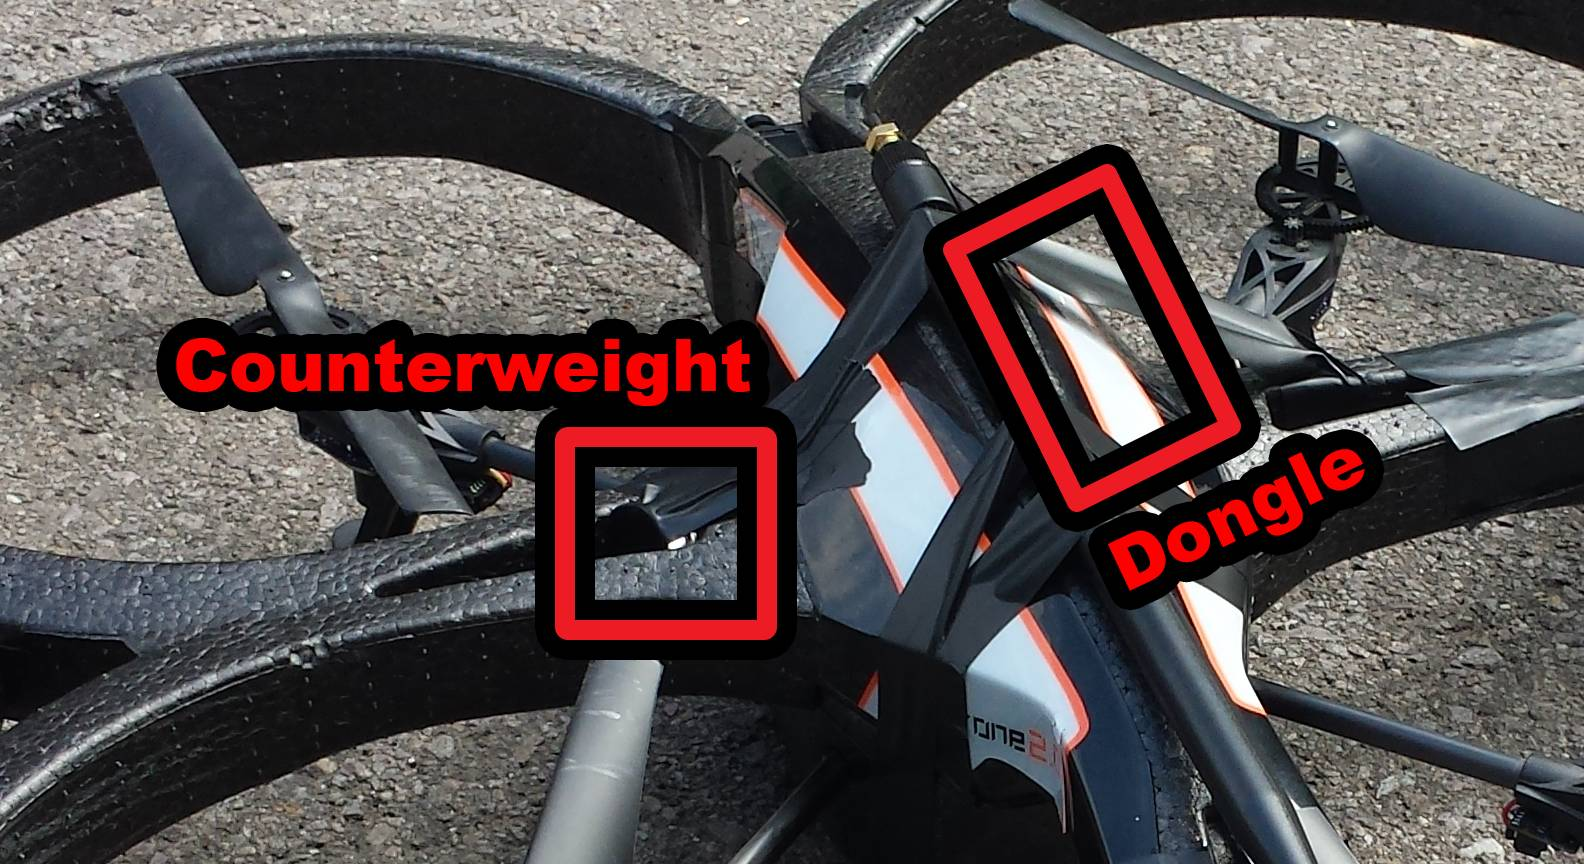
\includegraphics[width=0.9\textwidth]{img/counterweight.png}
\end{center}
\caption{\small \itshape{The counterweight needed to balance the drone}}
  \label{fig:counterweight}
\end{figure}


\section{The Sparrow family}

The Sparrow family, composed of the SparrowDongle and SparrowV3.2 shown in the figure~\ref{fig:sparrowfamily}, uses the 2.4 GHz band as a medium of communication. 
 

The main component of this family is the ATMega128RFA1\cite{atmegafa}. It is an 8-bit micro-controller from Atmel that has an on-chip 2.4 GHz wireless transceiver. On-chip transceivers occupy no extra PCB space and require little extra electronics to operate, making the footprint of the resulting boards very small. The on-chip transceiver allows more energy-efficient operating modes, and facilitates higher bandwidth transfers between the micro-controller's main memory and the transceiver frame-buffer, for a smaller power consumption.

\begin{figure}[ht]
\begin{center}
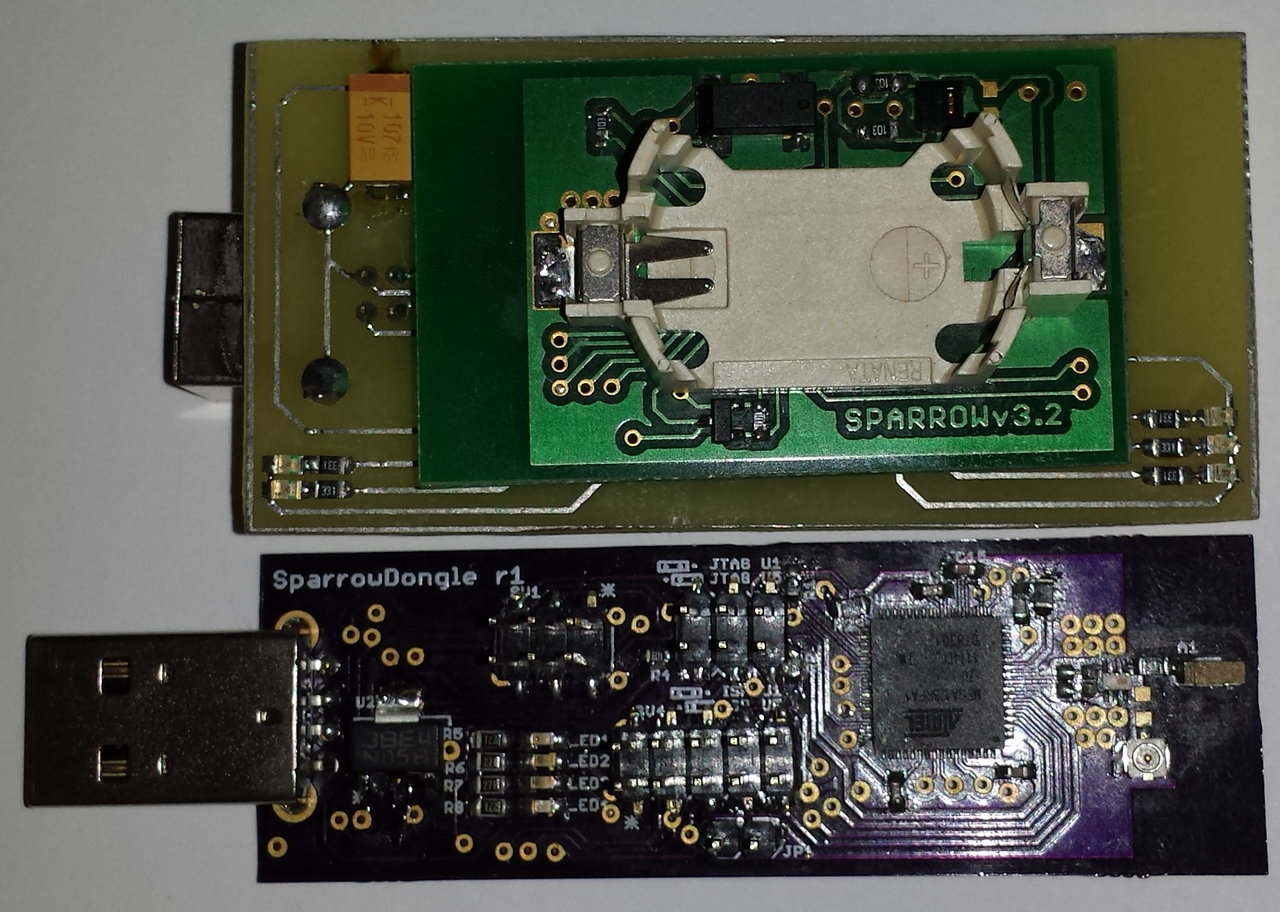
\includegraphics[width=0.9\textwidth]{img/sparrow.jpg}
\end{center}
\caption{\small \itshape{The SparrowDongle next to the SparrowV3.2}}
  \label{fig:sparrowfamily}
\end{figure}

The signal received or sent by the wireless transceiver can be boosted by attaching an external antenna. For example, in an ideal situation, with no interferences from the outside world, an 8 dBi omni-directional antenna mounted on both communication devices would amount to around 300 meters of communication range, well over the 70 meters measured with the default antennas.

This distance is achieved with the RX and TX at full power. A higher battery life can be achieved by reducing RX and TX power, but the maximum communication range will be shortened. The reduction can be compensated by installing a high gain antenna, but this can significantly increase the cost.

\subsection{The SparrowDongle}

\begin{figure}[ht]
\begin{center}
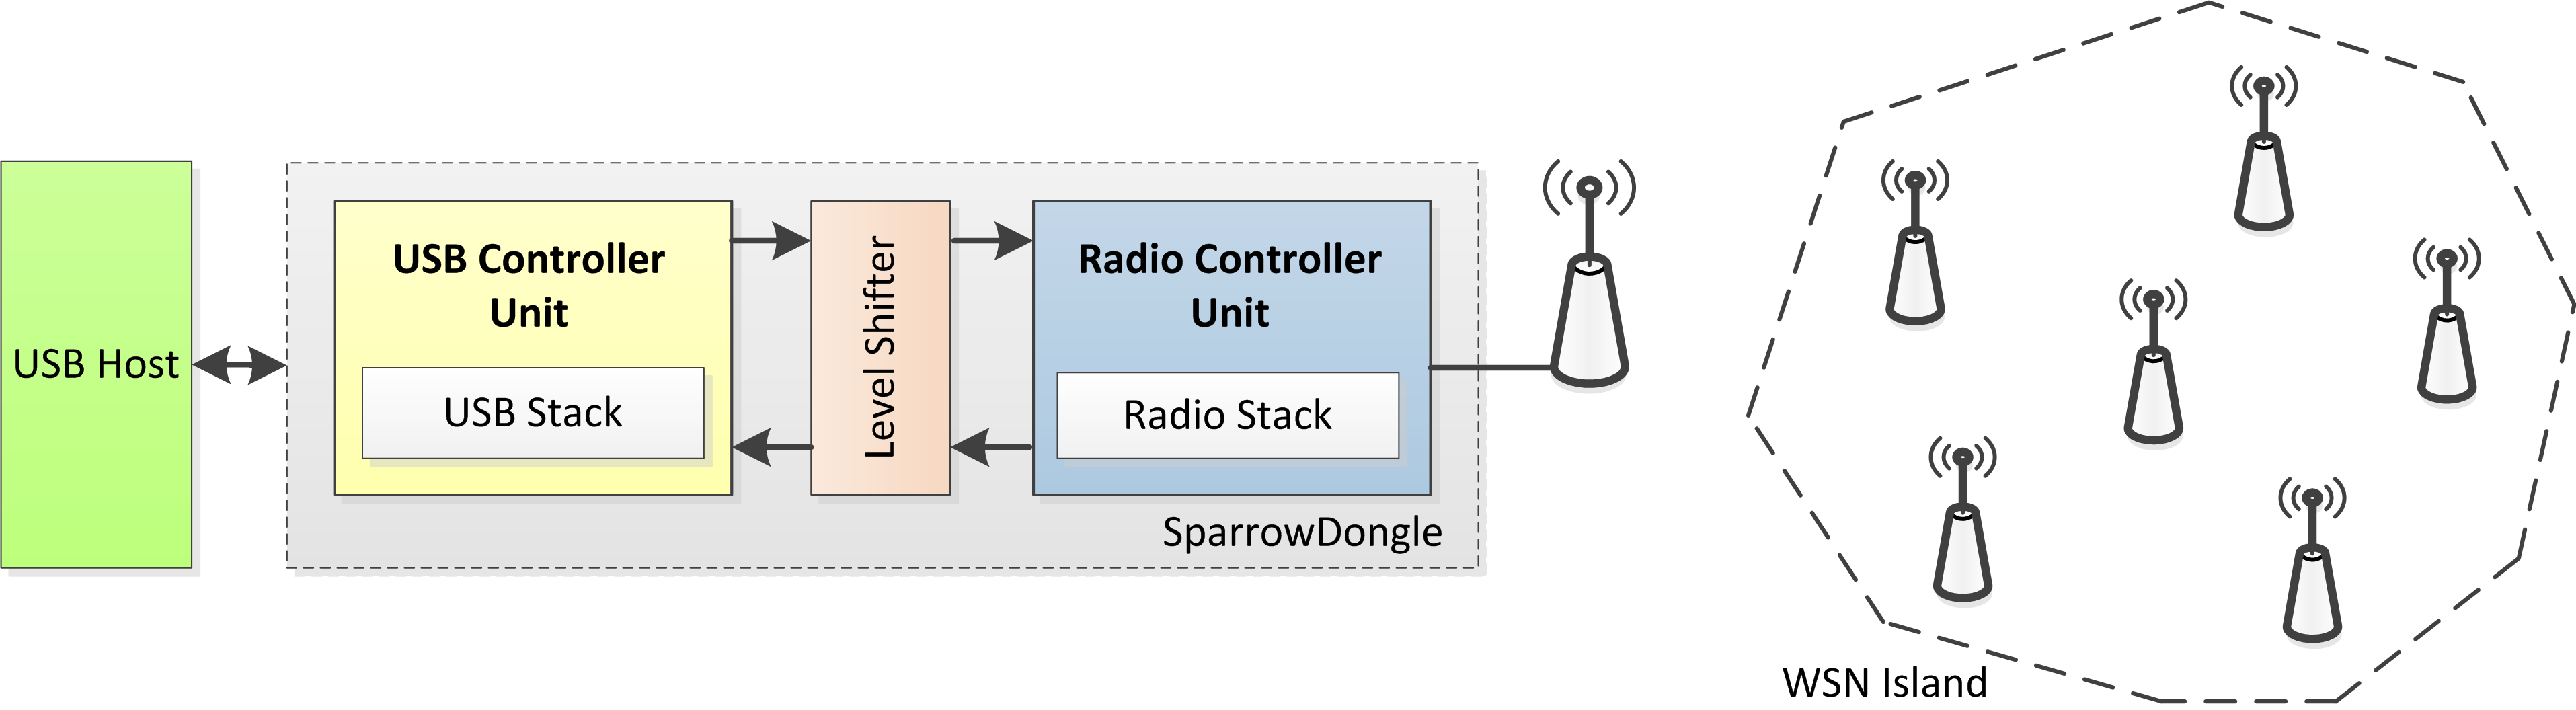
\includegraphics[width=0.9\textwidth]{img/donge_architecture.png}
\end{center}
\caption{\small \itshape{SparrowDongle stick architecture}}
\end{figure}
\footnotetext{Image taken from \cite{voinescu2013lightweight}}
 
The link between the wireless sensor networks and the rest of the digital world, the gateway of the Sparrow family is the SparrowDongle . The Dongle can be connected to any host that has an USB port and supports the USB CDC with ACM module (USB Communications Device Class with Abstract Control Mode). 

The dongle uses an ATmega32U4 as a dedicated USB Controller unit. This design allows the RF controller to run any RF communication stack without having the USB code intrude on key timings.\cite{voinescu2013lightweight}


\subsection{The SparrowV3.2}
 
 
The other member of the Sparrow family, the SparrowV3.2 node is responsible for collecting data from the surrounding environment and sending it to the SparrowDongle. The collected data depends on the sensors attached to the SparrowV3.2. The standard implementation has light, temperature and humidity sensors. Besides this information, the nodes also collect the battery level.

The SparrowV3.2 can be modified by adding additional sensors for a better measurement of environment parameters.

The node can be powered by a non-rechargeable battery, a rechargeable one or by a super-capacitor. Even though the super-capacitor can store only a small charge, the stored energy is sufficient enough to keep the node up and running for at least a day.

The advantages of the super-capacitor over the rechargeable battery are as follows:

\begin{itemize}
\item it can charge and discharge almost instantaneously 
\item it has a very high number of charge/discharge cycles 
\item it does not suffer from the same aging symptoms as a battery
\item it is far less pollutant than a standard battery
\item it will allow a longer maintenance-free time than a battery

\end{itemize}

The disadvantages of the super-capacitor are :

\begin{itemize}
\item it is bigger than a battery
\item it can store a much smaller amount of energy than similar sized batteries
\item it is very expensive
\item it operates at low voltages and may require a charge pump to rise the voltage

\end{itemize}

The rechargeable battery and/or the super-capacitor can be recharged from a solar panel, a wind turbine, or any other available source of energy.
